%--
\chapter{快速排序 (L4)}


%----------------------------------------
\section*{授课提纲}

%----------
\subsubsection{I - BF排序}

\nid 最朴素的\alg{SelectionSort}和\alg{BubbleSort}
%--
\begin{itemize}
    \item $W(n)$：$\choo{n}{2}$的必然性
    \item $A(n) = W(n)$
\end{itemize}
    
\nid \alg{InsertionSort}的改进
%--
\begin{itemize}
    \item 局部有序性的利用
    \item $W(n)$：不变
    \item $A(n)$：定量地降了一半
\end{itemize}
    
\nid 蛮力排序的不足
%--
\begin{itemize}
    \item inversion的概念
    \item inversion的数量：最多、平均
    \item 蛮力算法：消除inversion速度的不足
\end{itemize}

%----------
\subsubsection{II - 快速排序}

\nid 快速排序的设计原理
%--
\begin{itemize}
    \item 如何一次比较，消除更多的inversion
    \item 分治策略的典型应用：难分易合
\end{itemize}

\nid 快速排序的时间复杂度
\begin{itemize}
    \item $W(n)$：最不平衡的划分

    \item $A(n)$：列递归，解递归
    \begin{itemize}
        \item smart guess，guess \& prove
        \item 直接求解：错项相减
    \end{itemize}

    \item $A(n)$：指标随机变量、变量的linearality \footnote{将在tutorial（第\ref{chap:tut-divide-conquer}章）中专题讲解。}
\end{itemize}

%----------
\subsubsection{III - 空间复杂度}

\nid 空间复杂度的分档
%--
\begin{itemize}
    \item $O(1)$的含义：原地（in-place）排序
    \item $O(n)$的含义
\end{itemize}

\nid 蛮力排序、堆排序\footnote{将在相应课程（第\ref{chap:heap-sort}章）中针对性讲解。}
%--
\begin{itemize}
    \item 显然的$O(1)$空间
\end{itemize}

\nid 快速排序
%--
\begin{itemize}
    \item $O(n)$空间的朴素实现
    \item $O(1)$空间的改进：四个部分、一个不变式
\end{itemize}

\nid 归并排序：多次的反转 \footnote{将在相应课程（第\ref{chap:merge-sort}章）中针对性讲解。}
%--
\begin{itemize}
    \item 只能$O(n)$
    \item 可以$O(1)$
    \item 还是$O(n)$
\end{itemize}


%----------------------------------------
\section{快速排序}

%--------------------
\subsection{原地地划分的实现} \label{subsec:in-place-part}

在做\alg{Partition}的时候，开辟一个$O(n)$的辅助空间，划分很容易实现。
一个自然的想法是，能否将划分改为\ul{原地}（in-place）的。

原地划分的做法是，用两个指针$i$和$j$，将元素划分为四个部分，如图\ref{F:Partition}所示。
划分算法维护的不变式是$i$和$j$界定了小于部分和大于部分。

算法当前待处理的元素是$A[j]$。其他情况简单，唯一需要说明的是当$A[j]$纳入一个小于pivot的元素时，不变式被违反。

此时的做法很巧妙：让$i$指针右移一位，它也违反了不变式。
让$i$、$j$位置的元素互换，则两个违反都消失，整个数组恢复保持不变式。


%--
\begin{figure}[htbp]
    \center
    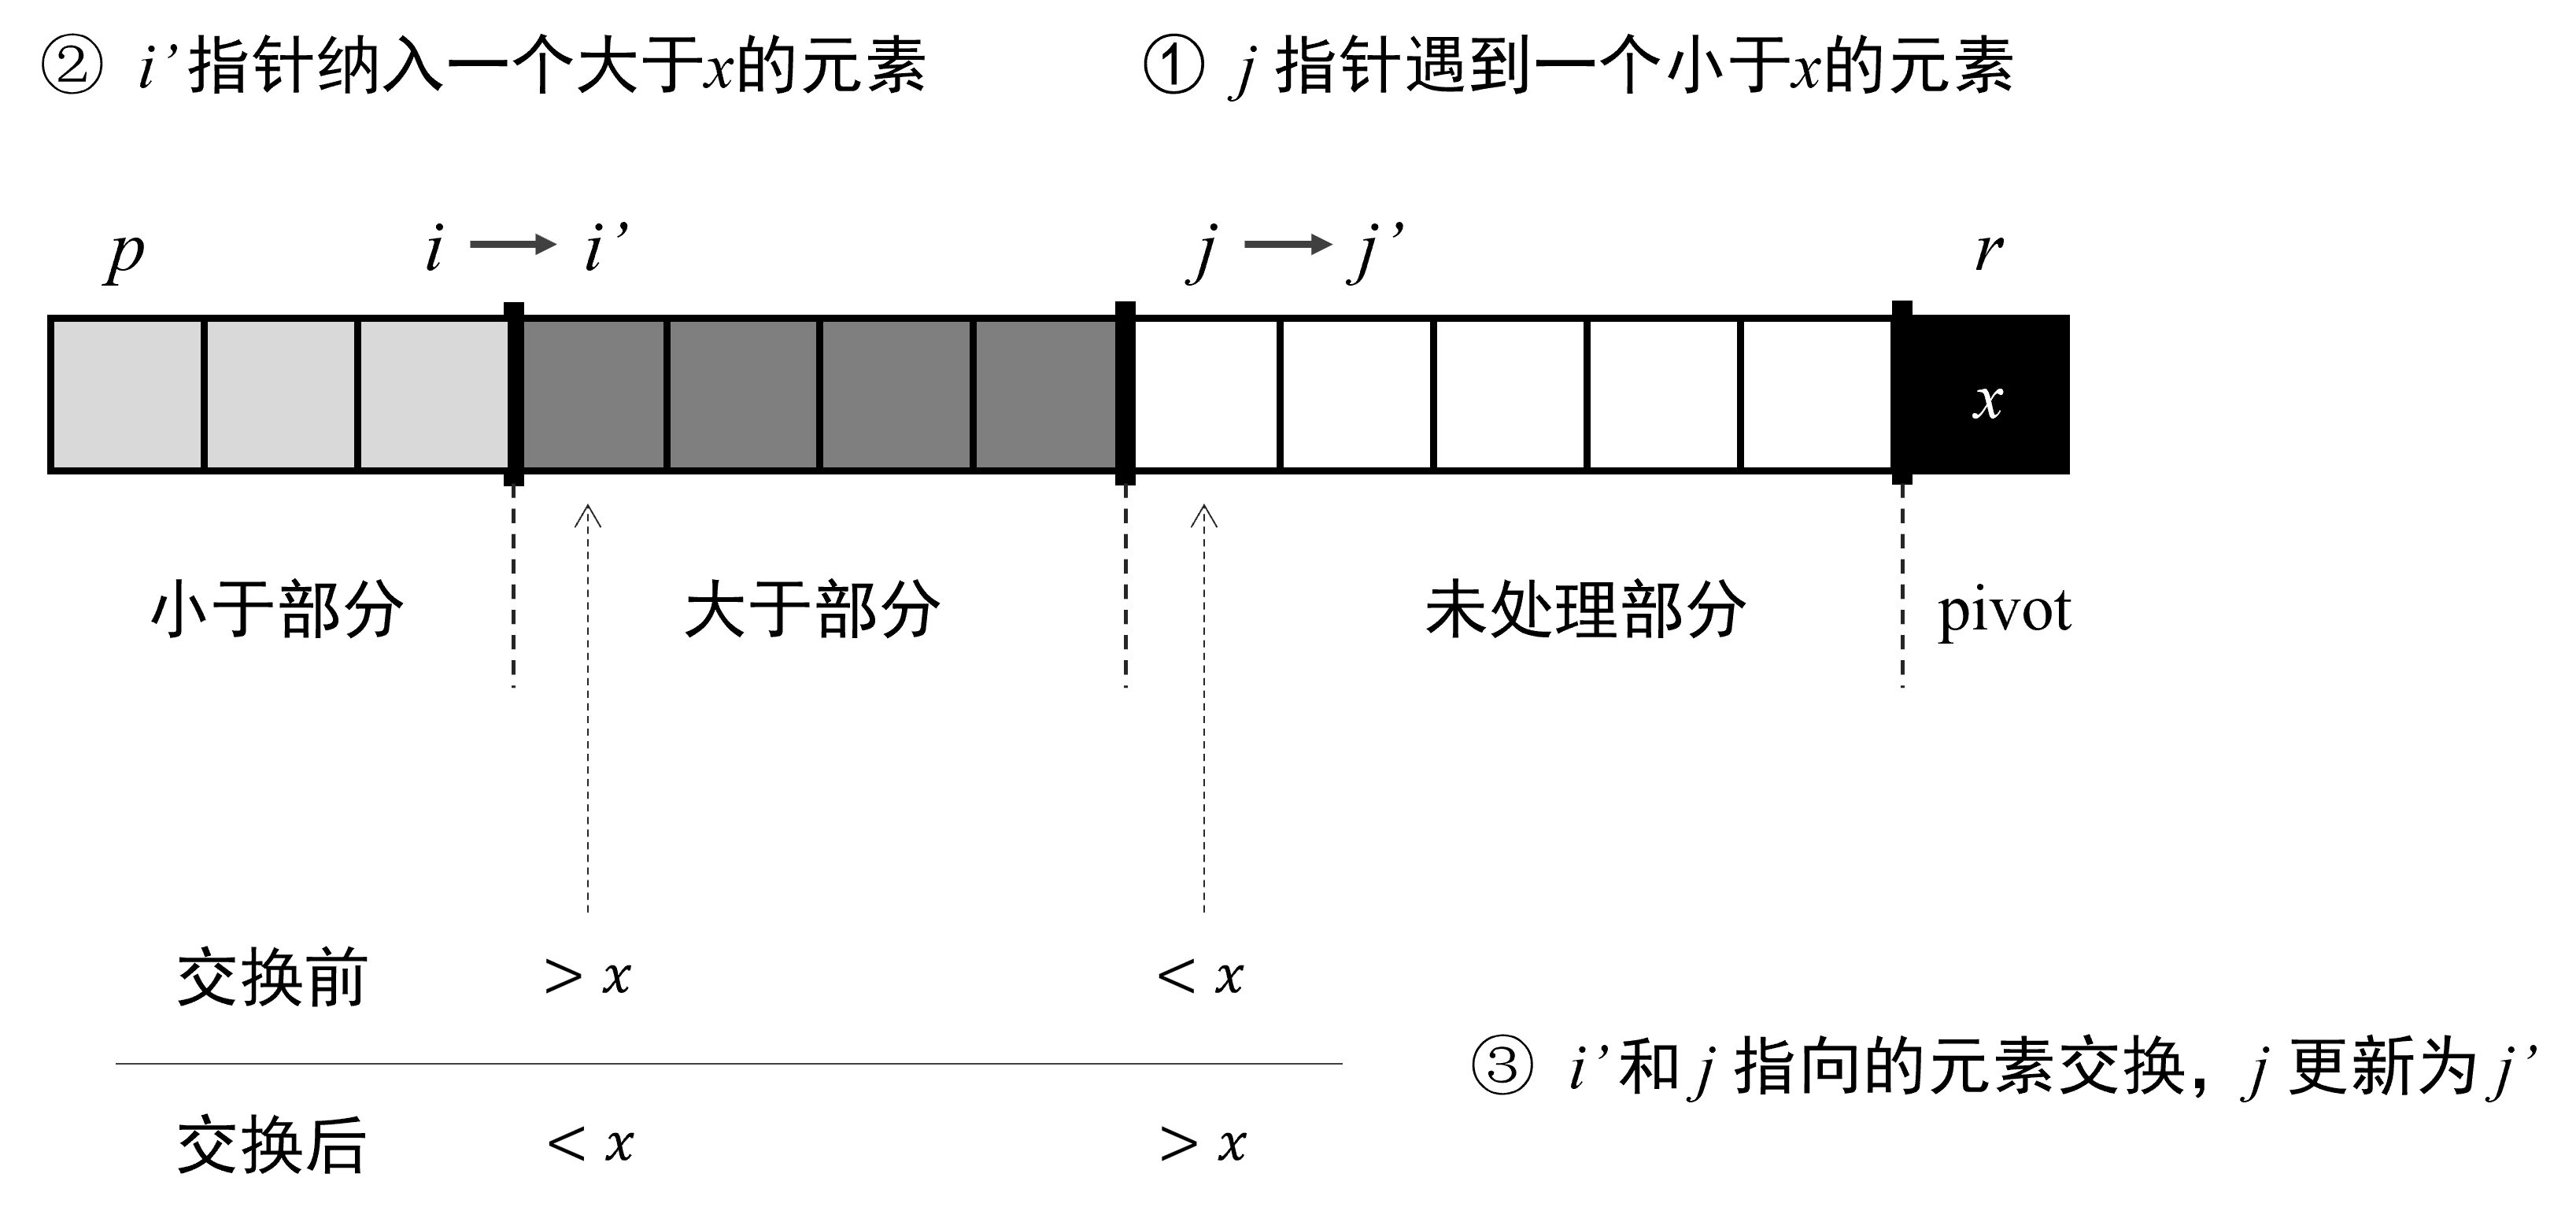
\includegraphics[width=0.8\columnwidth]{./figs/quick-sort/partition.png}
    \caption{原地的元素划分}
    \label{F:Partition}
\end{figure}